\maketitle
\setcounter{page}{1}
\newpage
\pagenumbering{arabic}
\section{Zielsetzung}
In der Festkörperphysik und Halbleitertechnik wichtige Informationen über die
Bandstruktur von Halbleitern können durch magneto-optische Untersuchungen gewonnen
werden. Insbesondere der $\textsc{Faraday}$-Effekt ist hierbei ein wichtiges
Messwerkzeug. Mithilfe dieses Effekts können effektive Massen von Halbleiterelektronen
bestimmt werden, was Ziel dieses Versuchs ist.

\section{Theorie}
\subsection{Effekive Masse}
\begin{figure}[H]
  \center
  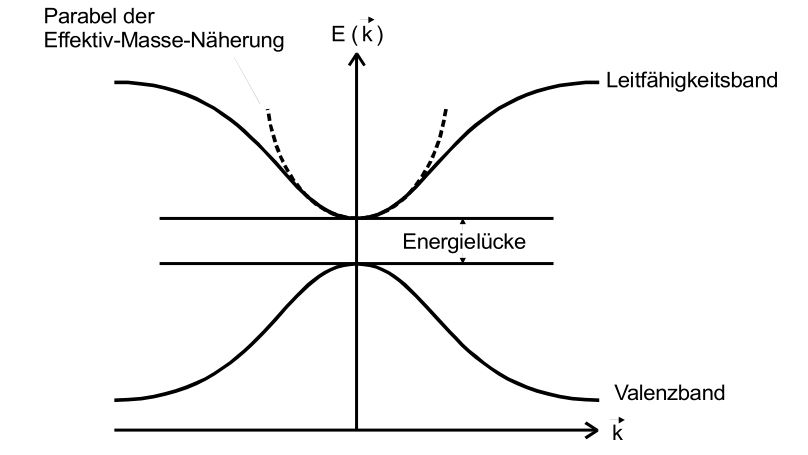
\includegraphics[width=0.4\textwidth]{Bilder/Energiebaender.jpg}
  \caption{Schematische Darstellung des Energiebandstruktur \cite{Anleitung}.}
  \label{T_Abb:1}
\end{figure}
Zur Beschreibung der Bandstruktur von Kristallen ist in es in vielen Fällen hinreichend,
sich auf die untere Bandkante der Energiebänder zu beschränken (siehe Abbildung \ref{T_Abb:1}).
Der Verlauf der Energiebänder (entspricht der Elektronenenergie) wird mit einer Funktion
$\varepsilon(\vec{k})$ durch den Wellenzahlvektror $\vec{k}$ beschrieben. Diese bei
Betrachtung des Gesammtverlaufs des Energiebandes in den meisten Fällen äußerst
komplizierte Funktion kann in der Nähe der Bandkante nach den Komponenten von $\vec{k}$
taylorentwickelt werden. Sinniger Weise wird die Bandkante dabei in den Nullpunkt
des Koordinatensystems gelegt, sodass um Null entwickelt werden kann. Es folgt eine Taylorreihe:
\begin{equation}
  \varepsilon(\vec{k}) = \varepsilon(0) + \frac{1}{2} \sum_{i=1}^3 \left(
  \pdv[2]{\varepsilon}{k_i} \right)_{k=0} k_i^2 + \mathcal{O}(k_i^3).
  \label{T_eq:1}
\end{equation}
Weiterhin gilt die Beziehung
\begin{equation*}
  \varepsilon = \frac{\hbar^2 k^2}{2 m}
\end{equation*}
und ein Vergleich mit der Taylorreihe zeigt, dass die Größen:
\begin{equation*}
  m_i^* \coloneq \hbar^2 \left\{ \left(\pdv[2]{\varepsilon}{k_i} \right)_{k=0} \right\}^{-1}
\end{equation*}
Massen beschreiben. Diese Größen werden effektive Massen genannt und ermöglichen es,
dass Kristallelektronen als freie Elektronen betrachtet werden, wenn ihre Ruhemassen
in der Schrödingergleichung mit eben diesen effektiven Massen ersetzt werden. Das
Potential wird dann durch die effektive Masse berücksichtigt und für mäßige externe
Felder gilt das 2. $\textsc{Newtonsche}$ Axiom.\\
Für perfekte Kristallsymmetrien vereinfacht sich die Taylorentwicklung \eqref{T_eq:1}
dergestalt, dass aus den offensichtlich elliptischen Energieflächen kugelsymmetrische
werden (in diesem Fall gilt $k_x = k_y = k_z$).
Für solche Flächen lässt sich der $\textsc{Faraday}$-Effekt beschreiben.

\subsection{Zirkulare Doppelbrechung bei optisch aktiver Materie}
\begin{figure}[H]
  \center
  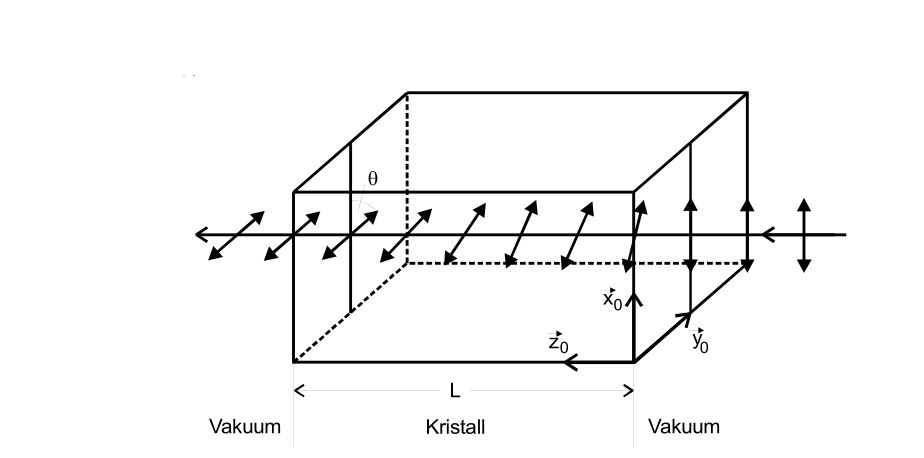
\includegraphics[width=0.4\textwidth]{Bilder/Kristall.jpg}
  \caption{Drehung der Polarisationsachse nach Durchgang durch ein optisch
  aktives Medium \cite{Anleitung}.}
  \label{T_Abb:2}
\end{figure}
Beim Eintreten eines linear polarisierten Lichtstrahls in ein optisch aktives Medium
wird die Polarisationsebene des Strahls gedreht. Dies lässt sich dadurch verstehen,
dass eine linear polarisierte Welle zu gleichen Teilen aus einem rechtszirkular und
einem linkszirkular zur Ausbreitungsrichtung (im folgenden $\vec{z}$) polarisierten
Teil besteht. Die beiden Zirkularisationsrichtungen breiten sich nun mit unterschiedlichen
Phasengeschwindigkeiten (bzw. Wellenzahlvektoren) aus und die linear polarisierte
Welle, die nach dem Durchgang durch den Kristall wieder austritt, ist um den Winkel $\theta$
gedreht (siehe Abbildung \ref{T_Abb:2}). Der Rotationswinkel berechnet sich zu
\begin{align*}
    \theta &=\frac{L}{2} \left(k_{\text{R}}-k_{\text{L}}\right)\\
          &=\frac{L\omega}{2}\left(\frac{1}{v_{\text{ph}_{\text{R}}}}-\frac{1}{v_{\text{ph}_{\text{L}}}}\right)\\
          &=\frac{L\omega}{2\text{c}}\left(n_{\text{R}}-n_{\text{L}}\right),
\end{align*}
wobei $v_{\text{ph}}=\omega k^{-1}$ die Phasengeschwindigkeit und $n=c v_{\text{ph}}^{-1}$
der Brechungsindex für links- bzw. rechtspolarisiertes Licht in einem Kristall der
Länge $L$ ist. Die Lichtfreuqenz der einlaufenden Welle ist durch $\omega$ gegeben.\\
Dieser, als zirkulare Doppelbrechung bezeichnete, Effekt geht auf im Kristallmedium induzierte
Dipole (permantente Dipole können der Frequenz des einfallenden Lichts nicht folgen) zurück.
Die Polarisation $\vec{P} = \varepsilon_0 \chi \vec{E}$ des Kristalls
steigt damit propotional zur dielektrischen Suszeptibilität
$\chi$. Für isotrope Materialien handelt es sich hier um eine skalare Größe, in anisotropen
Medien ist $\chi$ jedoch richtungsabhängig und muss daher tensoriell definiert werden.
In vielen Fällen handelt es sich hier um eine Diagonalmatrix, das Material ist dann
nicht doppelbrechend (optisch inaktiv). Doppelbrechende Materialien weisen jedoch Nebenachseneinträge
auf, sodass $\chi$ in einfachen Fällen eine Gestalt:
\begin{equation*}
    \underline{\underline{\chi}} =
    \begin{pmatrix}
      \chi_{\text{xx}} & i\chi_{\text{xy}} & 0 \\
      -i \chi_{\text{xy}}& \chi_{\text{xx}} & 0 \\
      0& 0 & \chi_{\text{zz}}
      \end{pmatrix}
\end{equation*}
annimmt. Für den Drehwinkel nach Durchgang folgt dabei nach Taylorentwicklung in
erster Ordnung in guter Näherung:
\begin{equation}
  \theta = \frac{L \omega}{2 c n} \chi_{xy}.
  \label{T_eq:2}
\end{equation}

\subsection{Zirkulare Doppelbrechung bei optisch inaktiver Materie}
Als $\textsc{Faraday}$-Effekt wird nun das Auftreten des oben beschriebenen Effekts
bei optisch inakiver Materie bezeichnet, wenn ein äußeres Magnetfeld angelegt wird.
Aus der Bewegungsgleichung für ein gebundenes Elektron folgt bei Vernächlässigung
von Dämpfungseffekten und Feldeinflüssen durch das Lichtfeld für hohe
Lichtfrquenzen eine Verschiebungspolarisoation $\vec{P} = -N e_0 \vec{r}$.
Es lässt sich nun das in \eqref{T_eq:2} benötigte Tensorelement $\chi_{xy}$ bestimmen
und in guter Näherung folgt:
\begin{equation*}
  \theta(\lambda)=\frac{2\pi^2 \text{e}_0^3 \text{c}}{\epsilon_0}\frac{1}{{m^*}^2
  \lambda^2 \omega{_0}^4}\frac{N B L}{n}.
\end{equation*}
Hierbei wird durch $N$ die Anzahl der Elektronen pro Volumeneinheit, durch $B$
die externe Magentfeldstärke, durch $\lambda$ die Wellenlänge des einfallenden
Lichts und durch $\omega_0$ die meist im nahen infraroten liegende Resonanzfrequenz
der zu erzwungenen Schwingungen fähigen gebundenen Elektronen bezeichnet. Weiter
lässt sich im Limes $\omega_0 \rightarrow 0$ (also für freie Elektronen) ein Ausdruck
\begin{equation}
  \theta_{\text{frei}}(\lambda)=\frac{\text{e}_0^3}{8 \pi^2 \epsilon_0 \text{c}^3}
  \frac{\lambda^2}{{m^*}^2}\frac{N L B}{n}
  \label{T_eq:3}
\end{equation}
entwickeln. Dieser kann unter Verwendung der oben eingeführten effektiven Masse
auch für Kristallelektronen verwendet und zur Bestimmung ebendieser genutzt werden.

\section{Durchführung}
\subsection{Versuchsaufbau}
\begin{figure}[H]
  \center
  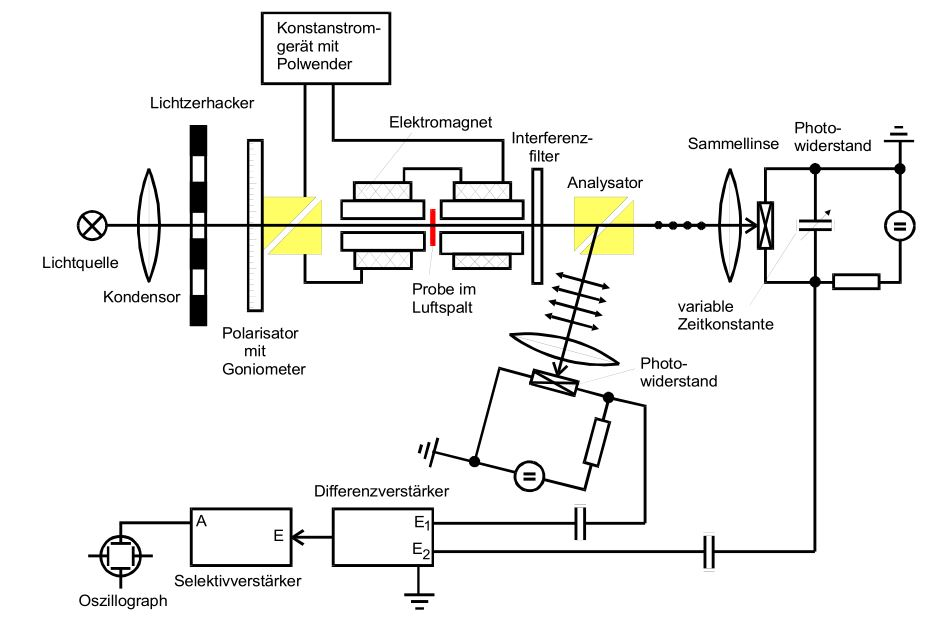
\includegraphics[width=0.8\textwidth]{Bilder/Aufbau.jpg}
  \caption{Schematische Darstellung des Versuchsaufbaus \cite{Anleitung}.}
  \label{D_Abb:1}
\end{figure}
Der Versuchsaufbau ist in Abbildung \ref{D_Abb:1} dargestellt. Das von einer Halogenlampe
emittierte Infrarotlicht wird über eine Kondensorlinse fokussiert,
durch einen Interferenzfilter monochromatisiert und durch
ein $\textsc{Glan-Thompson}$-Prisma (Polarisator) linear polarisiert. Die von diesem Licht durchleuchtete
Probe befindet sich dabei in einem Elektromagneten. Der Elektromagnet wird durch ein
Konstantspannungsgerät mit Strom versorgt. Nach Durchlauf durch den Magneten trifft der Lichtstrahl
auf ein weiteres $\textsc{Glan-Thompson}$-Prisma (Analysator), durch welches der Strahl aufgespalten wird.
Beide Strahlen werden durch Sammellinsen auf Photowiderstände abgebildet. Damit an
den Photowiderständen eine Wechselspannung abfällt, wird ein Lichtzerhacker in den Strahlgang
eingebracht. Die abfallenden Spannungen werden auf einen Differenzverstärker
gegeben, der einem Selektivverstärker vorgelagert ist. Letzterer ist an die
Frequenz des Zerhackers gekoppelt. Der Ausgang des Selektivverstärkers wird letztlich
auf einem Oszilloskop dargestellt.

\subsection{Versuchsdurchführung}
Zu Anfang muss der Aufbau ohne Interferenzfilter und Probe justiert werden.
Nun wird in folgender Reihenfolge vorgegangen:
\begin{enumerate}
  \item Justage des Analysator-Prismas:\\
  Das Analysator-Prisma wird so um seine vertikale Achse gedreht, dass
  der gerade durch das Prisma gehende Strahl bei geeigneter Stellung des
  Polarisator-Prismas verschwindet.
  \item Justage der Photowiederstände:\\
  Die relative Position zwischen den Photowiederständen und den vorgelagerten
  Sammellinsen wird so einjustiert, dass die einfallenden Strahlen gut auf
  die Photowiderstände abgebildet werden.
  \item Justage des Selektivverstärkers:\\
  Der Zerhacker wird eingeschaltet und die gewählte Frequenz am Selektivverstärker
  eingestellt. Der Differenzverstärker wird dafür durchgeschaltet. Das Ausgangssignal wird
  nun auf dem Oszilloskop beobachtet und  der Selektivverstärker zu eingeregelt,
  dass das Signal maximal wird.
  \item Helligkeitsjustage:\\
  Position von Lichtquelle und Linse werden so gewählt, dass die Lichtintensität
  besser wird.
  \item Überprüfen der Apperatur:\\
  Es werden Probe und Interferenzfilter eingesetzt und unter Variation von
  Polarisatorstellung und Zeitkonstante eines Photowiderstands geprüft,
  ob am Selektivverstärker ein Signal abfällt, dass, bis auf Störspannungen, null ist.
\end{enumerate}
Der Drehwinkel wird dabei bestimmt, indem die Polarisatorstellung und die Zeitkonstanten der
Photowiderstände abwechselnd so eingestellt werden, dass am Differenzverstärker eine Spannung
Null abfällt. Die Winkelstellung des Polarisators wird abgelesen und die Messung
bei umgepolten Magnetfeld widerholt. Der Drehwinkel ergibt sich dann zu:
\begin{equation}
  \theta = \frac{1}{2} \left(\theta_1 - \theta_2 \right).
  \label{runederaffe}
\end{equation}
Es wird der Drehwinkel an n-dotiertem und hochreinem Galliumarsenit für mehrere Wellenlängen
im nahen Infrarot gemessen.\\
Zuletzt wird das maximale Magnetfeld in Strahlrichtung mit einer Hallsonde gemessen.
\section{Auswertung}
\subsection{Bestimmung der Kraftflussdichte}
In Tabelle \ref{tab:1} sind die gemessenen Kraftflussdichten und der jeweilige
Ort $z$ aufgetragen. $z_\symup{rel}$ ist der Ort relativ zum Ort der Probe,
welcher in den Koordinatenursprung gelegt wurde. Außerdem befindet sich
der Plot und die Regression in Abbildung \ref{fig:2}.
\begin{figure}[p]
  \centering
  \subcaptionbox{Messwerte. \label{tab:1}}[0.4\textwidth]{
  \centering
  \begin{tabular}{c c c}
    \toprule
    $B(z)$ / \si{\milli\tesla} & $z$ / \si{\milli\meter} & $z_\symup{rel}$ / \si{\milli\meter} \\
    \midrule
    51 & 65 & -15\\
    188 & 70 & -10\\
    209 & 72 & -8\\
    219 & 74 & -6\\
    222 & 75 & -5\\
    224 & 76 & -4\\
    225 & 77 & -3\\
    226 & 78 & -2\\
    225 & 79 & -1\\
    225 & 80 & 0\\
    222 & 81 & 1\\
    219 & 82 & 2\\
    214 & 83 & 3\\
    209 & 84 & 4\\
    200 & 85 & 5\\
    187 & 86 & 6\\
    149 & 88 & 8\\
    90 & 90 & 10\\
    17 & 95 & 15\\
    \bottomrule
  \end{tabular}
  }
  \subcaptionbox{Grafische Darstellung mit Regression. \label{fig:2}}[0.58\textwidth]{
  \centering
  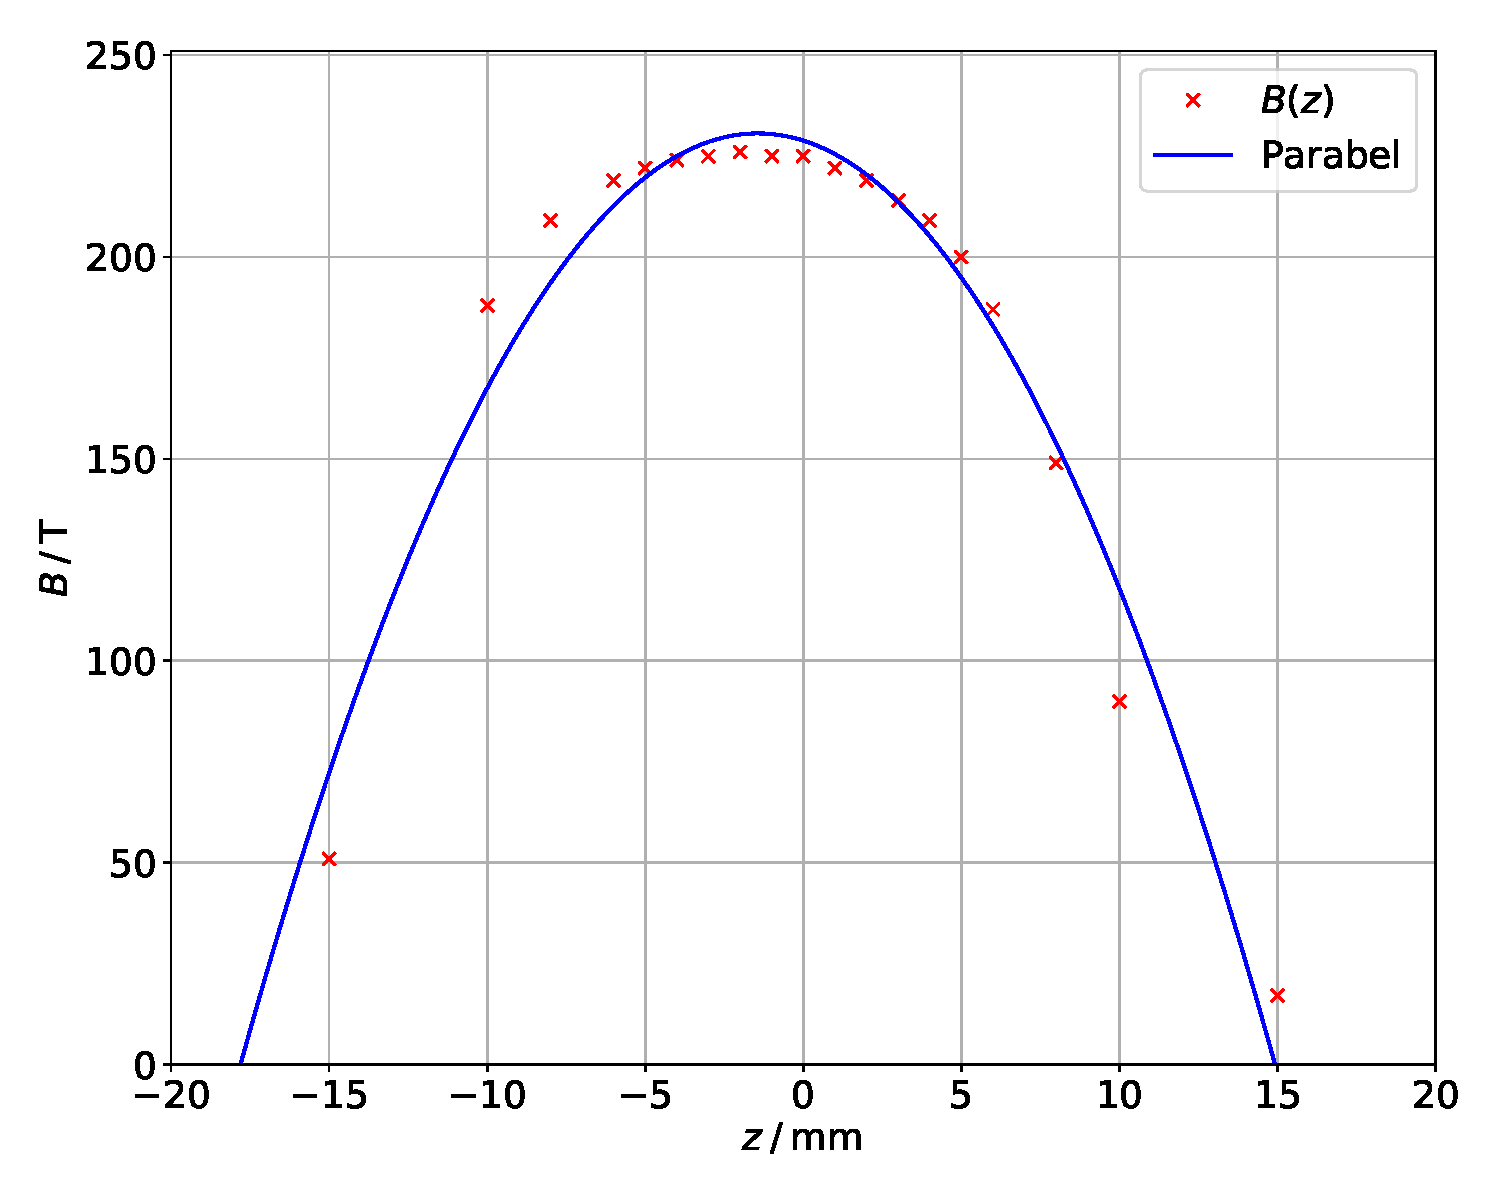
\includegraphics[width=0.58\textwidth]{BFeld.pdf}
  }
  \caption{Kraftflussdichte $B(z)$ in Abhängigkeit vom Ort $z$.}
  \label{fig:1}
\end{figure}


Mit der Funktion
\begin{equation}
  f(x) = a \, x^2 + b \, x + c
  \label{eqn:1}
\end{equation}
und $B(z)$ und $z_\symup{rel}$ wird eine Augleichsrechnung gemacht. Es ergibt sich
\begin{align*}
  a &= \SI{-0.86(4)}{\tesla\per\meter^2} \\
  b &= \SI[per-mode=reciprocal]{-2.5(4)}{\tesla\per\meter} \\
  c &= \SI{229(4)}{\tesla} \\
\end{align*}
für die Parameter. Das Maximum dieser Parabel liegt bei $B_\symup{max} = \SI{231(4)}{\milli\tesla}$.
\subsection{Drehwinkel des hochreinen und des n-dotierten GaAs}
Für alle gemessenen Winkel wird nach \eqref{runederaffe} der Drehwinkel
bestimmt. Jene Drehwinkel zusammen mit der jeweiligen Wellenlänge und dem
längennormierten Winkel stehen in den Tabellen \ref{tab:2} bis \ref{tab:4}.
Die Normierungen wurden mit den angegebenen Längen in den Tabellen durchgeführt.
\begin{table}
  \centering
  \caption{Wellenlänge, $\theta_1$ und $\theta_2$, der daraus berechnete
  Drehwinkel und längenormierter Drehwinkel für
  hochreines GaAs mit $L$ = \SI{5.11e-3}{\meter}.}
  \label{tab:2}
  \begin{tabular}{c | c c | c c}
    \toprule
    $\lambda$ / \si{\micro\meter} & $\theta_1$ / \si{\degree} & $\theta_2$ / \si{\degree} &
    $\theta$ / \si{\degree} & $\theta_\symup{norm}$ /
    \si{\degree\per\meter} \\
    \midrule
    1.29 & 149.23 & 138.67 & 5.28 & 1033.92 \\
    1.06 & 332.33 & 310.42 & 10.96 & 2144.49 \\
    1.45 & 327.33 & 311.37 & 7.98 & 1562.30 \\
    2.16 & 336.00 & 330.08 & 2.96 & 578.93 \\
    2.34 & 2.92 & -0.42 & 1.67 & 326.16 \\
    2.51 & 210.83 & 198.00 & 6.42 & 1255.71 \\
    2.65 & 164.00 & 158.78 & 2.61 & 510.44 \\
    1.72 & 148.22 & 139.78 & 4.22 & 825.18 \\
    \bottomrule
  \end{tabular}
\end{table}

\begin{table}
  \centering
  \caption{Wellenlänge, $\theta_1$ und $\theta_2$, der daraus berechnete
  Drehwinkel und längenormierter Drehwinkel für
  das erste n-dotierte GaAs mit $N$ = \SI{1.2e18}{\per\cubic\centi\meter}
  und $L$ = \SI{1.36e-3}{\meter}.}
  \label{tab:3}
  \begin{tabular}{c | c c | c c}
    \toprule
    $\lambda$ / \si{\micro\meter} & $\theta_1$ / \si{\degree} & $\theta_2$ / \si{\degree} &
    $\theta$ / \si{\degree} & $\theta_\symup{norm}$ /
    \si{\degree\per\meter} \\
    \midrule
    1.29 & 143.67 & 136.23 & 3.72 & 2732.84 \\
    1.06 & 143.93 & 133.45 & 5.24 & 3854.17 \\
    1.45 & 143.53 & 137.00 & 3.27 & 2401.96 \\
    2.16 & 150.83 & 145.58 & 2.62 & 1930.15 \\
    2.34 & 179.97 & 171.90 & 4.03 & 2965.69 \\
    2.51 & 209.93 & 202.55 & 3.69 & 2714.46 \\
    2.65 & 260.25 & 252.75 & 3.75 & 2757.35 \\
    1.72 & 273.53 & 267.18 & 3.18 & 2334.56 \\
    \bottomrule
  \end{tabular}
\end{table}
  \begin{table}
    \centering
    \caption{Wellenlänge, $\theta_1$ und $\theta_2$, der daraus berechnete
    Drehwinkel und längenormierter Drehwinkel für
    das zweite n-dotierte GaAs mit $N$ = \SI{2.8e18}{\per\cubic\centi\meter}
    und $L$ = \SI{1.296e-3}{\meter}.}
    \label{tab:4}
    \begin{tabular}{c | c c | c c}
      \toprule
      $\lambda$ / \si{\micro\meter} & $\theta_1$ / \si{\degree} & $\theta_2$ / \si{\degree} &
      $\theta$ / \si{\degree} & $\theta_\symup{norm}$ /
      \si{\degree\per\meter} \\
      \midrule
      1.29 & 275.73 & 267.25 & 4.24 & 3272.89 \\
      1.06 & 278.08 & 267.05 & 5.52 & 4256.69 \\
      1.45 & 143.75 & 136.20 & 3.78 & 2912.81 \\
      2.16 & 155.02 & 142.27 & 6.38 & 4918.98 \\
      2.34 & 181.23 & 168.62 & 6.31 & 4867.54 \\
      2.51 & 212.17 & 205.67 & 3.25 & 2507.72 \\
      2.65 & 161.32 & 153.50 & 3.91 & 3015.69 \\
      1.72 & 146.47 & 138.83 & 3.82 & 2944.96 \\
      \bottomrule
    \end{tabular}
\end{table}
\clearpage
In Abbildung \ref{fig:3} sind sich die längennormierten Drehwinkel gegen das
Quadrat der Wellenlängen aufgetragen.
\begin{figure}
  \centering
  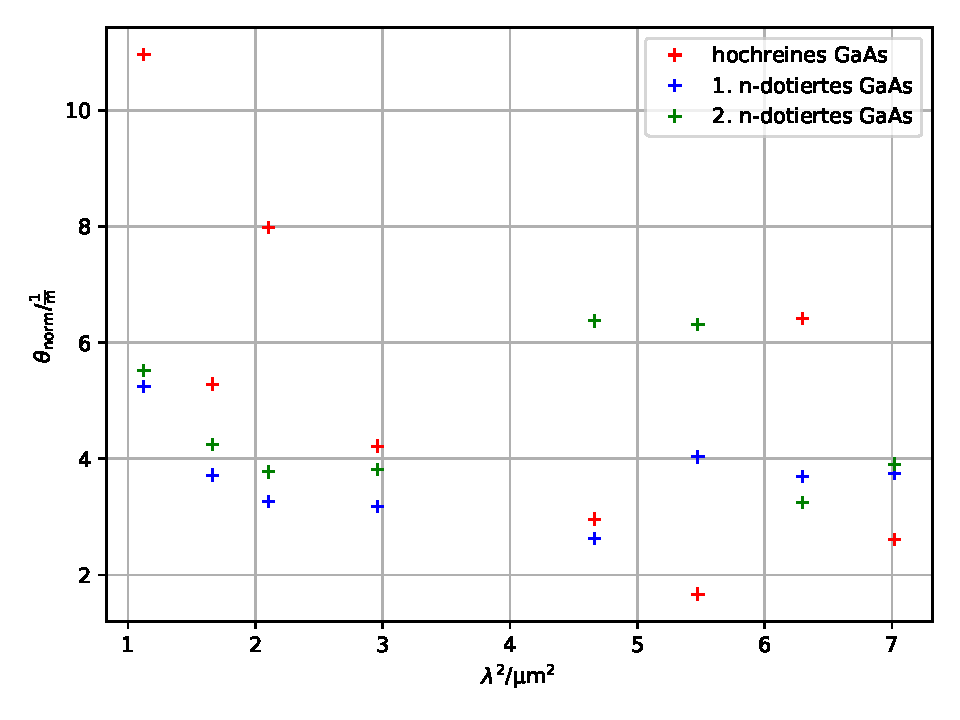
\includegraphics[scale=0.5]{b.pdf}
  \caption{Die längennormierten Winkel gegen $\lambda ^2$ aufgetragen.}
  \label{fig:3}
\end{figure}
\subsection{Bestimmung der effektiven Masse}
Zur Bestimmung der effektiven Masse werden die Differenzen zwischen den
$\theta_\symup{norm}$ des hochreinen GaAs und der beiden n-dotierten GaAs
gebildet.
Diese befinden sich in Tabelle \ref{tab:5}. Außerdem wird eine lineare Ausgleichrechnung
durchgeführt, nach der Form
\begin{equation*}
  g(x) = m \, x + b \, .
\end{equation*}
Diese ist in Abbildung \ref{fig:5} dargestellt. Es ergeben sich
\begin{align}
  m_1 &= \SI{1.1(9)e2}{\per\cubic\meter} \label{eqn:2} \\
  b_1 &= \SI{1.2(4)e3}{\per\meter}
\end{align}
für die erste Regression und
\begin{align}
  m_2 &= \SI{1.6(22)e2}{\per\cubic\meter} \label{eqn:3} \\
  b_2 &= \SI{1.9(1)e3}{\per\meter}
\end{align}
für die zweite Regression. Um nun die effektive Masse zu bestimmen, wird
\eqref{T_eq:3} genutzt. Aufgrund der Regression gilt
\begin{equation}
  m_{1, 2} = \frac{\text{e}_0^3}{8 \pi^2 \epsilon_0 \text{c}^3}
  \frac{1}{{m^*}^2}\frac{N B}{n} \, .
  \label{eqn:4}
\end{equation}
Umgestellt ergibt sich aus \eqref{eqn:4}
\begin{equation}
  m^* = \sqrt{\frac{\text{e}_0^3}{8 \pi^2 \epsilon_0 \text{c}^3}
  \frac{1}{m_{1, 2}}\frac{N B}{n}}
  \label{eqn:5}
\end{equation}
für die effektive Masse. Für $N$ und $B$ werden die bereits erwähnten Größen
eingesetzt und für den Brechungsindex der Wert $n =$ 3.3543\footnote{aus \cite{n}}
für $\lambda =$ \SI{1771.14}{\nano\meter}, da der Mittelwert unserer Wellenlängen
bei \SI{1897.5}{\nano\meter} liegt. Es ergeben sich
\begin{align*}
  m_\symup{eff, 1} &= \SI{1.9(7)e-33}{\kilo\gram} \\
  m_\symup{eff, 2} &= \SI{1.1(7)e-33}{\kilo\gram}
\end{align*}
und
\begin{align*}
  \frac{m_\symup{eff, 1}}{\symup{m_e}} &= \num{0.0021(8)} \\
  \frac{m_\symup{eff, 2}}{\symup{m_e}} &= \num{0.0012(8)} \, .
\end{align*}
Als Mittelwert ergibt sich
\begin{equation}
  \frac{m_\symup{eff}}{\symup{m_e}} = \num{0.0016(6)} \, .
  \label{eqn:6}
\end{equation}

\begin{figure}[h]
  \centering
  \subcaptionbox{Messwerte. \label{tab:5}}[0.35\textwidth]{
  \centering
  \begin{tabular}{c c}
    \toprule
    $\theta_1$ & $\theta_2$ \\
    \midrule
    1698.92 & 2238.97 \\
    1709.68 & 2112.20 \\
    839.66 & 1350.51 \\
    1351.22 & 4340.05 \\
    2639.53 & 4541.38 \\
    1458.75 & 1252.01 \\
    2246.92 & 2505.25 \\
    1509.38 & 2119.78 \\
    \bottomrule
  \end{tabular}
  }
  \subcaptionbox{Grafische Darstellung mit Regression. \label{fig:5}}[0.6\textwidth]{
  \centering
  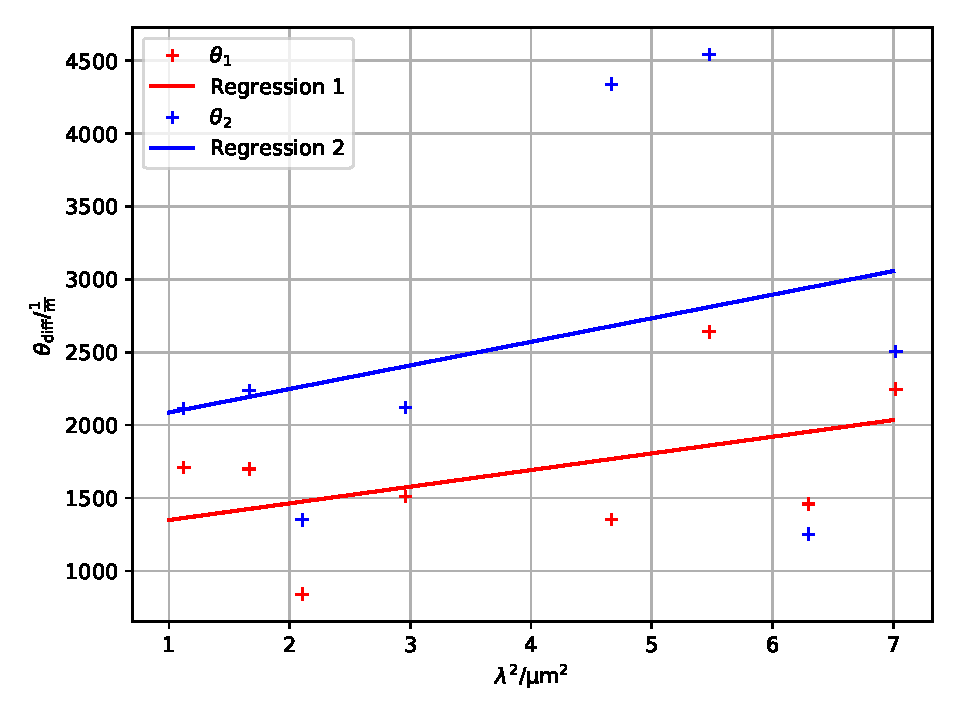
\includegraphics[width=0.6\textwidth]{Test.pdf}
  }
  \caption{Der Drehwinkel der Leitungselektronen gegen die Wellenlänge
  zum Quadrat aufgetragen.}
  \label{fig:4}
\end{figure}

\subsection{Fehlerrechnung}
Die Fehlerrechnung wird in $\textsc{Python}$\footnote{\cite{python}} durchgeführt.
Mittelwerte werden durch die Funktion $\textsc{mean}$ aus dem Paket $\textsc{Numpy}$\footnote{\cite{numpy}},
die zugehörigen Standartabweichungen durch die Funktion $\textsc{stats.sem}$ aus dem
Paket $\textsc{scipy}$\footnote{\cite{scipy}} berechnet. Fehlerfortpflanzung wird
durch die Bibliothek $\textsc{uncertainties.unumpy}$\footnote{\cite{uncertainties}} berechnet
mit der Gaußschen Fehlerfortpflanzungsformel
\begin{equation}
    \symup \Delta f(x_1, x_2, ..., x_n) = \sqrt{\left(\frac{\symup df}{\symup dx_1} \symup \Delta
    x_1 \right)^2 +    \left(\frac{\symup df}{\symup dx_2} \symup \Delta
    x_2 \right)^2 + ... + \left(\frac{\symup df}{\symup dx_n} \symup \Delta x_n \right)^2} \ .
    \label{fehler}
\end{equation}
Fehlerbehaftete Größen sind das mittels Augleichsrechnung bestimmte Maximum der
Kraftflussdichte, die Steigungen $m_1$ und $m_2$ der Differenzen der $\theta_\symup{norm}$
und alles, was aus diesen
Winkeln bestimmt wird. Damit ergibt sich \eqref{fehler} zu
\begin{equation}
    \symup \Delta m^*(B, m_{1, 2}) = \sqrt{\left(\frac{\symup dm^*}{\symup dB} \symup \Delta
    B \right)^2 +    \left(\frac{\symup dm^*}{\symup dm_{1, 2}} \symup \Delta
    m_{1, 2} \right)^2} \ .
    \label{fehler2}
\end{equation}

\section{Diskussion}
\subsection{Zur Berechnung der Kraftflussdichte}
Die Bestimmung der Kraftflussdichte hat insgesamt gut funktioniert.
Es wird aus \ref{fig:2} ersichtlich, dass die Regression verhältnismäßig gut
an die Werte angepasst ist. Das Maximum, um dessen Bestimmung es ging, ist gut
approximiert worden.
\subsection{Zur Bestimmung der Drehwinkel}
Die Bestimmung der Drehwinkel ist eher schlecht verlaufen, wie aus \ref{fig:3}
ersichtlich wird. Es ist kein linearer Verlauf zu erkennen. Genauer gesagt ist
keine Korrelation zwischen den Messwerten zu erkennen, was vor allem durch das große
Rauschen durch den sich erwärmenden und daraufhin im infraroten Bereich abstrahlenden
Elektromagneten und die damit verbundene sehr unterschiedliche Minimumsbestimmung
am Differentialverstärker. Außerdem wurde die Bestimmung des Minimums dadurch erschwert,
dass für höhere Wellenlängen die Interferenzfilter nur noch sehr wenig Licht durchgelassen
haben und damit ein zu kleines Signal an den Differenzverstärker gelangte.
\subsection{Zur Bestimmung der effektiven Masse}
Auch die Bestimmung der effektiven Masse ist eher schlecht verlaufen. In Abbildung
\ref{fig:5} ist ebenfalls nur mit viel gutem Willen ein linearer Verlauf zu erkennen,
auch sind die Regressionen nicht ganz parallel. Die Gründe dafür liegen in der
fehlerhaften Bestimmung der Drehwinkel, da diese in die Rechnung bzw. den Fit
eingeflossen sind. Vor diesem Hintergrund ist die relative Abweichung von 97.6\% vom
Literaturwert\footnote{aus \cite{lit}} $\frac{m_\symup{eff}}{\symup{m_e}} = 0.067$
einfach einzusehen. Unser berechneter Wert liegt eine Größenordnung unter dem
Literaturwert, was unter den Umständen verständlich ist. \\
\\
Zum Abschluss lässt sich sagen, dass bis auf die Bestimmung der Kraftflussdichte
die bestimmten Werte stark von den Literaturwerten abweichen. Allerdings war
der Aufbau nicht ganz optimal, die Photowiderstände ließen sich verbessern,
sodass diese auch bei weniger Intensität
trotzdem noch ein starkes Signal an den Differentialverstärker geben. Weiterhin
waren die Interferenzfilter teilweise verschmutzt und ließen dadurch auch weniger
Intensität passieren. Mit einer Optimierung des Aufbaus ließe sich die effektive
Masse bzw. die Faraday-Rotation besser bestimmen. Allein für die Einführung des
Faraday-Effekts und seiner Anwendungen in der heutigen Halbleiterindustrie
war der Versuch sehr anschaulich und einfach durchzuführen.

\newpage
\nocite{*}
\printbibliography
